\documentclass[11pt]{article}
\PassOptionsToPackage{dvipsnames}{xcolor}
\usepackage{amsmath, amssymb, amscd, amsthm, amsfonts}
\usepackage{tikz}
\usetikzlibrary{math}
\usetikzlibrary{positioning}
\usepackage{comment}
\usepackage{circuitikz}
\usepackage{graphicx}
\usepackage{hyperref}
\usepackage{amssymb}
\usepackage[makeroom]{cancel}
\oddsidemargin 0pt
\evensidemargin 0pt
\marginparwidth 40pt
\marginparsep 10pt
\topmargin -20pt
\headsep 10pt
\textheight 8.7in
\textwidth 6.65in
\linespread{1.2}

\title{APEX holography reduction pipeline}
%\author{Sebastian Jorquera}
\date{}

\newtheorem{theorem}{Theorem}
\newtheorem{lemma}[theorem]{Lemma}
\newtheorem{conjecture}[theorem]{Conjecture}

\newcommand{\rr}{\mathbb{R}}

\newcommand{\al}{\alpha}
\DeclareMathOperator{\conv}{conv}
\DeclareMathOperator{\aff}{aff}

\begin{document}

\maketitle

%\begin{abstract}

%\end{abstract}

\section{Nearfield Holography math background}

Our pipeline is mostly based on the Baars paper \cite{baars}, in this section a short mathematical review will be presented with the key concepts used in our holography pipelines.


The standard expression that links the radiation pattern $f(x,y,z)$ at a given point $P$ with the field distribution in $F(\epsilon, \nu)$ at the aperture plane is given by the equation \ref{eq:holo_general} where you can see the geometry and the parameters used in the equation in the figure \ref{fig:antenna_holo}.


\begin{equation}
    f(x,y,z) = \int \frac{F(\xi,\eta)}{4\pi r} e^{-ikr} \left[ \left(ik+\frac{1}{r} \right) \hat{z}\cdot r_1 + ik\hat{z}\cdot\hat{s} \right] d\eta d\xi 
    \label{eq:holo_general}
\end{equation}


\begin{figure}
    \centering
    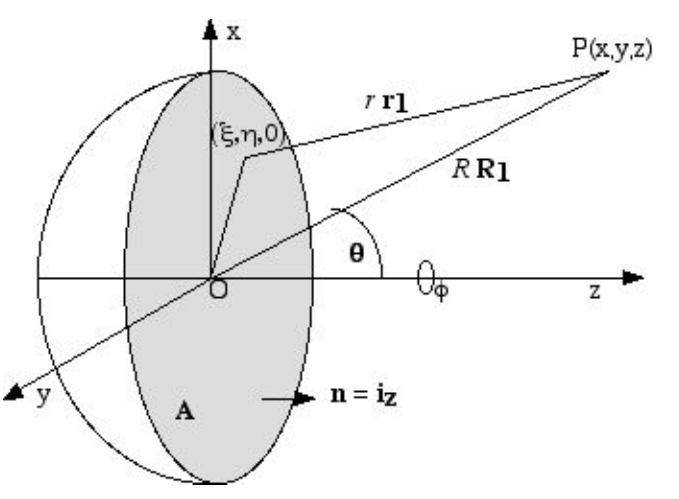
\includegraphics[width=0.5\textwidth]{images/antenna_holo.png}
    \caption{Geometry, parameters and variables used in the mathematical description.}
    \label{fig:antenna_holo}
\end{figure}


To simplify the problem some assumptions are commonly used:
\begin{enumerate}
    \item $\frac{1}{r} << k$
    \item $\frac{1}{r} \sim \frac{1}{R}$. This is not valid for the phase terms (ie the ones inside the bracket and in the exponential).
    \item  The term $\hat{z}\cdot r_1$ can be replaced by $\hat{z}\cdot R = \cos(\theta)$
    \item The term $\hat{z}\cdot \hat{s}$ represent the deviation from the uniform phase over the aperture. If the deviation is small the term can be considered to be 1.
\end{enumerate}

With all these assumptions the equation \ref{eq:holo_general} is transformed into equation \ref{eq:holo_assumptions}, where we defined $r= \sqrt{(x-\xi)^2+(y-\eta)^2+z^2}$.

\begin{equation}
f(x,y,z) = \frac{i}{2\lambda R}\int F(\xi,\eta)[\cos(\theta)+1]e^{ikr}d\eta d\xi
    \label{eq:holo_assumptions}
\end{equation}


\subsection{Far field approximation}
In the far field assumption, R tends to infinity, $R_1$ and $r_1$ are parallel then you could express $r=R-(u\xi+v\eta)$ and for a high gain antenna the interesting region is confined to small values of $\theta$ so we can  use $\cos(\theta)=1$. Then,  the equation \ref{holo_assumptions} is approximated to \ref{eq:holo_fourier}, which is a 2D Fourier transform in the aperture. So, with a given aperture distribution we are able to compute the far field using a Fourier transform. 


\begin{equation}
    f(u,v) = \frac{i}{\lambda}\frac{e^{-ikR}}{R} \int F(\xi,\eta)e^{-ik(\xi u+\eta v)} d\xi d\eta
    \label{eq:holo_fourier}
\end{equation}


The opposite is also true, we are able to compute the fields at the aperture if we measure the beam pattern. If we do that we would obtain a complex aperture $F(\xi, \eta)=A(\xi, \eta)$ and we can compute the surface errors related with the aperture phase with the equation \ref{eq:aperture2surface}. Where $\epsilon_n$ is the error normal to the surface and $F$ is the foci of the antenna. If we disregard the geometry the error is given by the Ruze formula shown in \ref{eq:ruze}

\begin{equation}
    \epsilon_n(\xi,\eta) = \frac{\lambda}{4\pi} \phi(\xi,\eta)\sqrt{1+\frac{\xi^2+\eta^2}{4F^2}}
    \label{eq:aperture2surface}
\end{equation}


\begin{equation}
    \phi = \frac{4\pi}{\lambda}\epsilon
    \label{eq:ruze}
\end{equation}


These ideas are the fundamental building blocks for the holography method to adjust an antenna:
\begin{enumerate}
    \item Make an Beam map measurement, obtaining the magnitude and phase of the signal. Typically this is done using a second antenna that is being used as reference.
    \item Compute the aperture distribution using the Fourier transform relation.
    \item Compute the surface errors on the antenna and calculate the adjustment of the panels.
\end{enumerate}


\subsection{Nearfield effects}
In this case we need to consider the phase variation in the aperture, ie the exponential terms cannot be simplified leading to a Fresnel diffraction integral shown in \ref{eq:holo_fresnel}.


\begin{equation}
    \frac{i}{\lambda}\frac{e^{ikR}}{R} \int F(\xi,\eta) exp\left(ik\left[-(u\xi+v\eta)+\frac{\xi^2+\eta^2}{2R}\right]\right)d\xi d\eta
    \label{eq:holo_fresnel}
\end{equation}


 In this case the approximation used is : $r \approx R-(u\xi+v\eta)+\delta p_1(\xi,\eta)+\epsilon$, where $\delta p_1$ contains terms that does not depends on the integration variables as shown in equations \ref{eq:holo_p1} and \ref{eq:holo_p2}.

\begin{equation}
    \delta p_1(\xi,\eta) = \frac{\xi^2+\eta^2}{2R}+\frac{(\xi^2+\eta^2)^2}{8R^3} \\
    \label{eq:holo_p1}
\end{equation}
\begin{equation}
    \epsilon = -\frac{(u\xi+v\eta)^2}{2R}+\frac{(\xi^2+\eta^2)(u\xi+v\eta)}{2R^2}
    \label{eq:holo_epsilon}
\end{equation}



To account the defocus of the telescope another term is added to $\delta p_1$, shown in the equation \ref{eq:holo_p2} where $f$ is the focal distance of the antenna and $\delta f$  is the variation of such distance.

\begin{equation}
    \delta p_2(\xi, \eta) = (\xi^2+\eta^2+(f-\frac{\xi^2+\eta^2}{4f}+\delta f)^2)^{1/2} - (f+\frac{\xi^2+\eta^2}{4f}+\delta f)
    \label{eq:holo_p2}
\end{equation}



With all these approximation the relation between the beam pattern and the aperture can be written as equation \ref{eq:holo_nearfield}, which for us is the most important equation for us.


\begin{equation}
    \boxed{ F(\xi, \eta) = \frac{i}{\lambda}\frac{e^{-ikR}}{R} exp\left(-ik[\delta p_1(\xi,\eta)+\delta p_2(\xi, \eta)]\right) \int f(u,v)exp\left(ik(u\xi+v\eta)\right)e^{-ik\epsilon} }
    \label{eq:holo_nearfield}
\end{equation}


The term $\epsilon$ can be expanded in a Taylor serie as shown in the equation \ref{eq:holo_taylor}. Depending on the accuracy that you need to met, when solving the equation \ref{eq:holo_nearfield} you can neglect some high order terms. Its good to note that the first term of the resulting equation recovers the Fourier transform relation, while the rest of the terms are modifications of the field that dissapears when $r$ is large enough.

\begin{equation}
    e^{-ik\epsilon} \approx 1-ik\epsilon = 1-ik\left[ u \frac{\xi(\xi^2+\eta^2)}{2R^2} + v \frac{\eta(\xi^2
+\eta^2)}{2R^2}-u^2\frac{\xi^2}{2R}-v^2\frac{\eta^2}{2R}-uv\frac{\xi\eta}{R} \right]
    \label{eq:holo_taylor}
\end{equation}



\subsection{Zernike polynomials}
Since the final goal of a radio holography measurement is to compute the adjustment of the panels that forms the primary reflector, we need to isolate the errors that comes from the single panel position and rule out the large scale errors that are present in the telescope, like for example optical aberrations. 


Zermike polynomials are a sequence of orthogonal polynomials on the unitary disk. They are used to describe different types of aberrations on optics. 
One advantage of the zernike polynomials is that they can be normalized, so the value of each component is proportional to the overall effect on the surface error.



The Zernike polynomils in the unit circle can be represented by the equations \ref{eq:zernike_eq} and \ref{eq:zernike_radial}. In the figure \ref{fig:zernike_pols} the first Zernike terms are shown.


\begin{equation}
    U_{n}^{m}(\rho, \theta) = \begin{cases}
        R_{n}^{m}(\rho)\cos(m \theta) & m \ge 0 \\
        R_{n}^{m}(\rho)\sin(m \theta) & m < 0
    \end{cases}
    \label{eq:zernike_eq}
\end{equation}

\begin{equation}
    R_{n}^{m}(\rho) = \frac{1}{\left(\frac{n-m}{2} \right) \rho^m} \left( \frac{d}{d(\rho^2)} \right)^{\frac{n-m}{2}} \left[ \left(\rho^2 \right)^{\frac{n+m}{2}} \left( \rho^2-1 \right)^{\frac{n-m}{2}} \right]
    \label{eq:zernike_radial}
\end{equation}



\begin{figure}
    \centering
    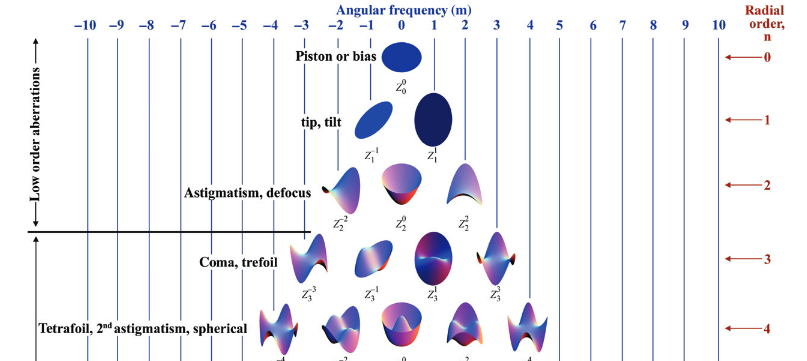
\includegraphics[width=0.9\textwidth]{images/zernike_pols.png}
    \caption{First Zernike polynomials.}
    \label{fig:zernike_pols}
\end{figure}












\section{APEX holography setup}

\section{Beam pattern to aperture conversion}

In this section the aim is to solve the equation \ref{eq:holo_nearfield}. We will separate the problem in two parts as shown in the equations \ref{eq:nearfield_reduced} and \ref{eq:fourier_like_integral}.


\begin{equation}
    \label{eq:nearfield_reduced}
    F(\xi, \eta) = \frac{i}{\lambda}\frac{e^{-ikR}}{R} exp\left(-ik[\delta p_1(\xi,\eta)+\delta p_2(\xi, \eta)]\right) \cdot \Phi(\xi, \eta)
\end{equation}
\begin{equation}
    \label{eq:fourier_like_integral}
    \begin{split}
        \Phi(\xi, \eta) = \int f(u,v)exp\left(ik(u\xi+v\eta)\right) \cdot \Biggl(1-ik\biggl[ u \frac{\xi(\xi^2+\eta^2)}{2R^2} + \\
        v \frac{\eta(\xi^2 +\eta^2)}{2R^2}-u^2\frac{\xi^2}{2R}-v^2\frac{\eta^2}{2R}-uv\frac{\xi\eta}{R} \biggr] \Biggr)
    \end{split}
\end{equation}

Since the distance of the APEX holography transmitter is at $1835m$, the first thing to investigate is if we need to solve numerically the integral shown in \ref{eq:fourier_like_integral} or if we just can take the first order approximation and compute the 2D Fourier integral using a Fast Fourier transform algorithm.


The current pipeline has the option of use both methods, but when applying them to the collected data the error atributted to the high order terms is neglectable. The figures \ref{fig:high_order_terms_power} and \ref{fig:high_order_terms_power_diff} shows the magnitude of the bona fide fourier transform and the high order integral terms in one of the APEX holography measurements. The figure \ref{fig:high_order_terms_power_diff} shows that the biggest effect of the high order terms are around the edges of the telescope, but even there the difference between the bona fide Fourier transform is $30dB$ higher than the values given by the high order integral terms.


We also had run the pipeline using the complete with and without considering the high order terms and the final difference in the RMS surface error maps is in the order of the $nm$ as its shown in the figure \ref{fig:high_fft_surf_error}


\begin{figure}
    \centering
    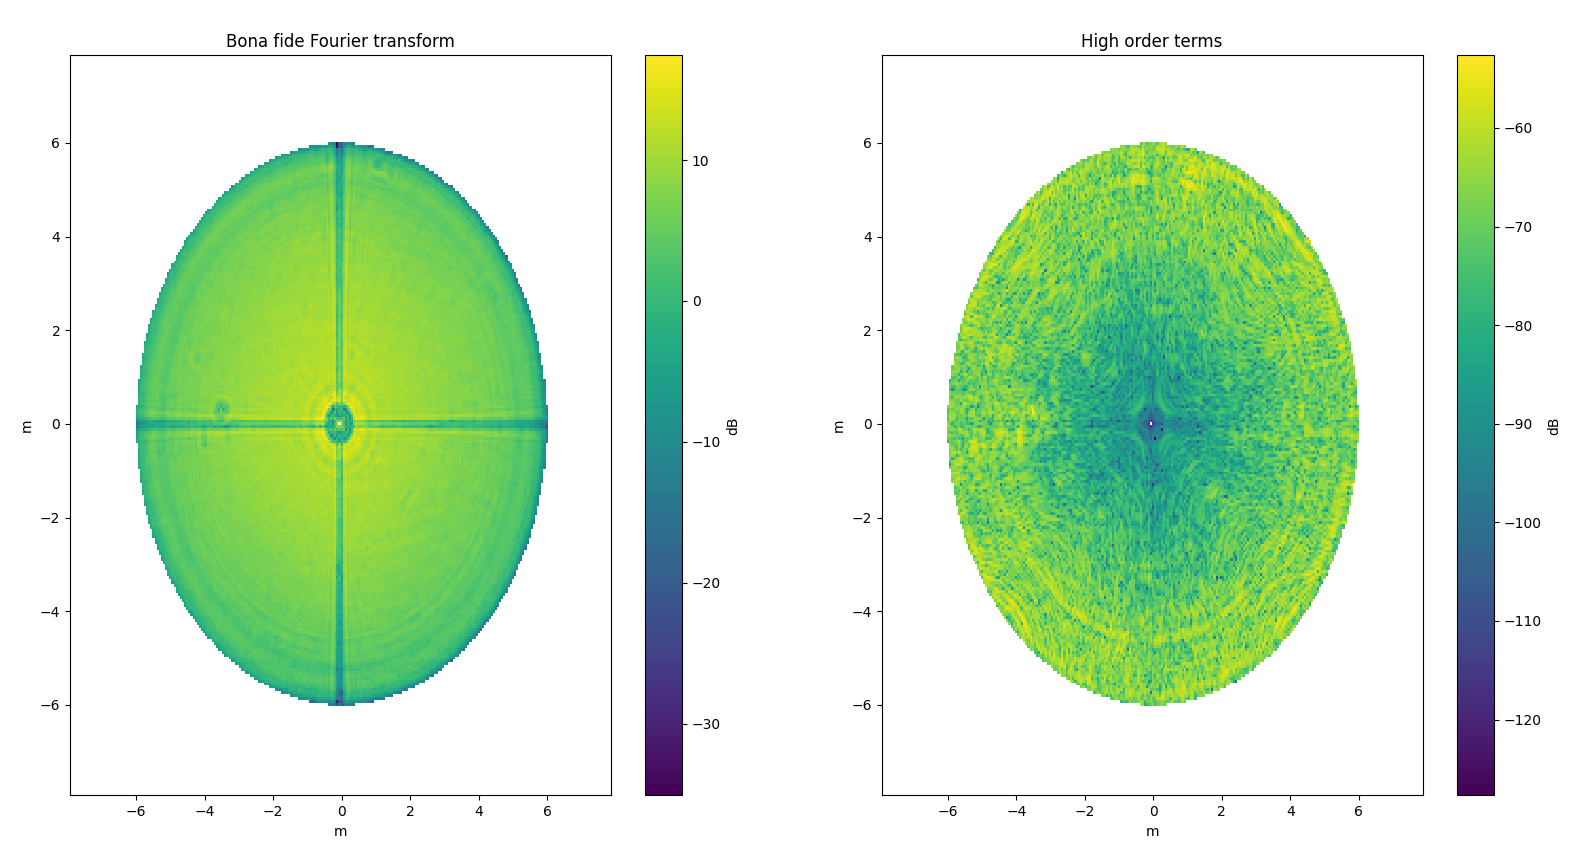
\includegraphics[width=1\textwidth]{images/high_order_fft.png}
    \caption{Power of the bona fide Fourier transform and the high order integral terms. Note that the scales are different for each map otherwise the image will be completly saturated.}
    \label{fig:high_order_terms_power}
\end{figure}


\begin{figure}
    \centering
    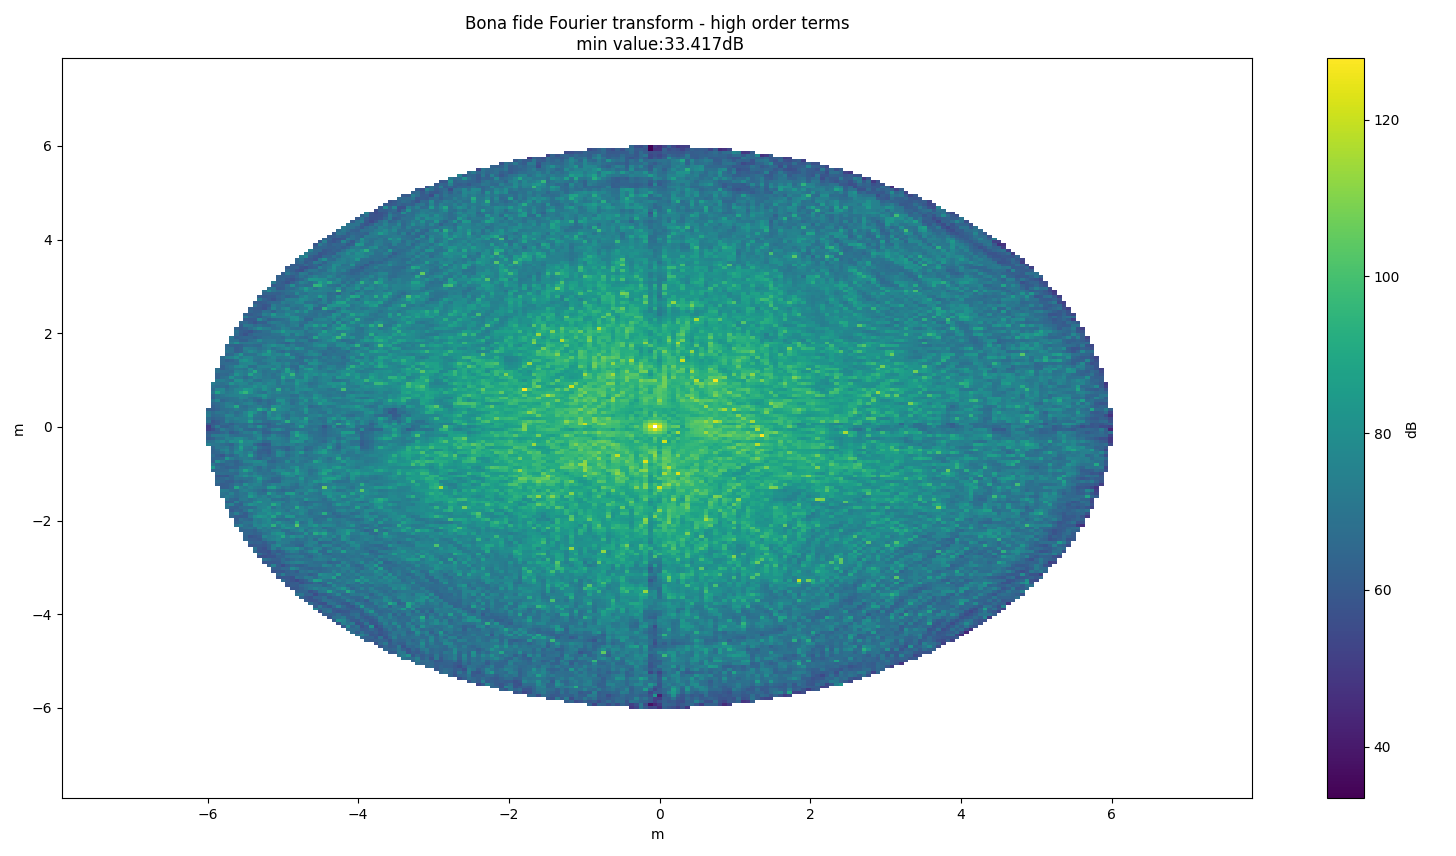
\includegraphics[width=0.9\textwidth]{images/fft_high_order_difference.png}
    \caption{Power difference of bona fide Fourier transform and the high order integral terms.}
    \label{fig:high_order_terms_power_diff}
\end{figure}


\begin{figure}
    \centering
    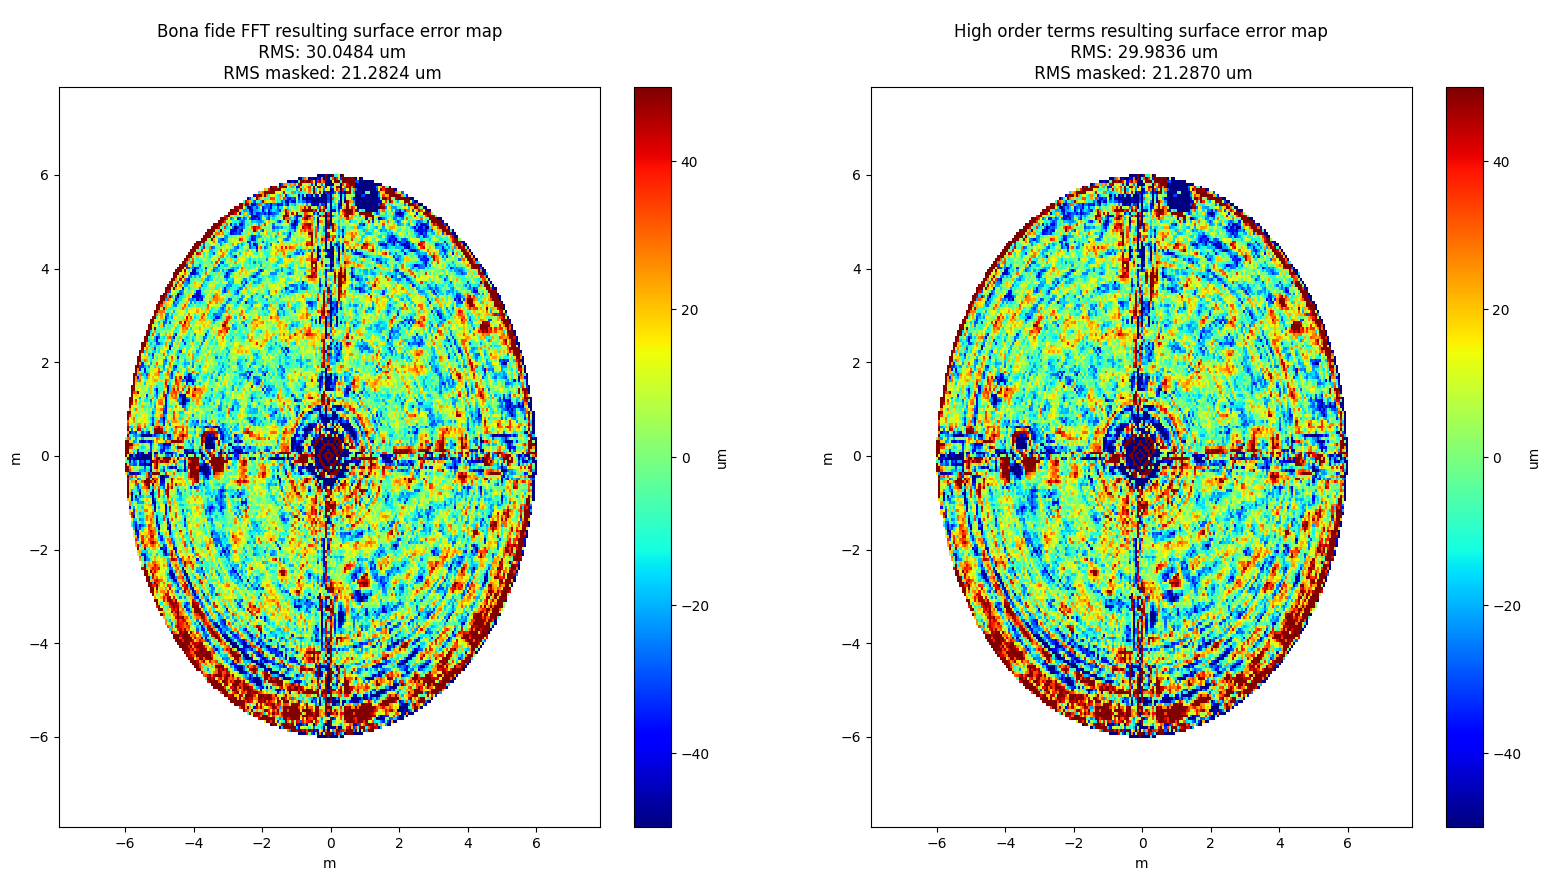
\includegraphics[width=1\textwidth]{images/high_vs_fft_surf_error.png}
    \caption{Final map given by the current pipeline considering solving the complete integral or just sticking with the Fourier transform. The final RMS difference is in the $nm$ scale.}
    \label{fig:high_fft_surf_error}
\end{figure}




\subsection{Defocus, Nearfield and tilt correction}
The defocus and nerafield corrections are contained in the $\delta p_1$ and $\delta p_2$ terms, where we need to find the proper $\delta f$ that match the measurements. Aditionally the measurement could have a tilt in the measure that needs to be removed. The tilting of a field can be generated by the equation \ref{eq:aperture_tilt}.

To find the parameters $(\delta f, \theta_x, \theta_y)$ we run an optimization process where the target is found the parameters that minimize the RMS surface error.

\begin{equation}
    E_{tilted}(x,y) = E(x,y)\exp\left(\frac{2\pi}{k}i\left(\theta_x\cdot x+ \theta_y \cdot y\right)\right)
    \label{eq:aperture_tilt}
\end{equation}


The figure \ref{fig:nearfield_correction} shows an example of the before and after of the corrections.



\begin{figure}
    \centering
    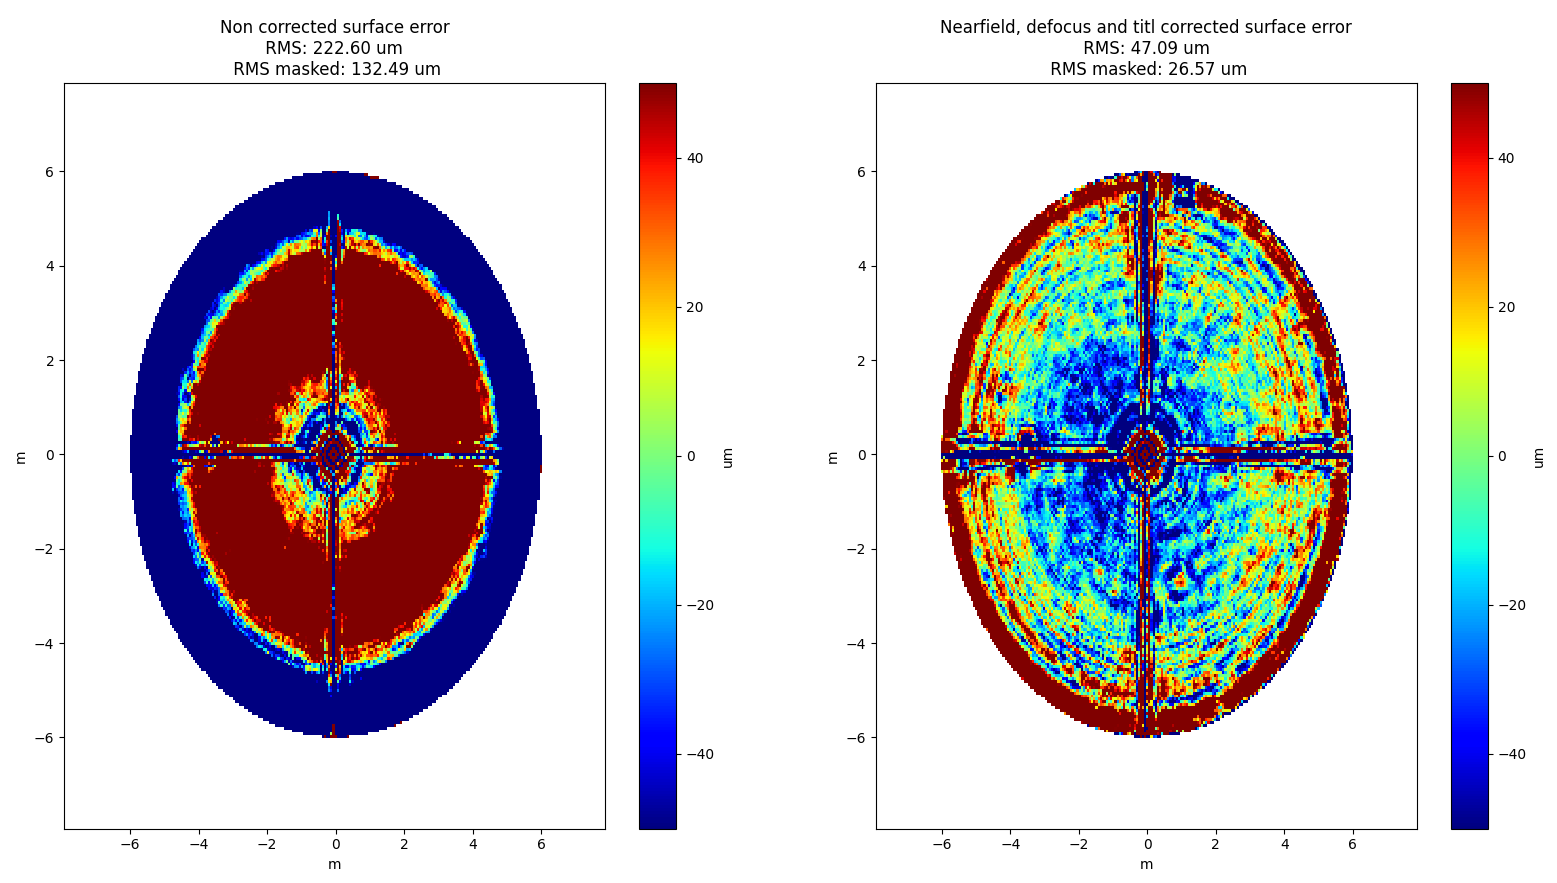
\includegraphics[width=1\textwidth]{images/nearfield_correction.png}
    \caption{Defocus, nearfield and tilt corrections. For this map the defocus and tilt values found by the optimization process were $\delta f = -15.36mm$, $\theta_x=-1.36arcsec$, $\theta_y =-1.41arcsec$}.
    \label{fig:nearfield_correction}
\end{figure}




\subsection{Aperture plane reference}

The position of the aperture plane would also induce RMS noise in the computed surface error. This is given by the geometrical transformation given in \ref{eq:aperture2surface} where implicitly there is a translation from a plane to a parabola, and the way that the plane fold will depend on the height of the plane itself with respect to the parabola. In the practical standpoint, the reference of the aperture position is given by the position where the zero phase is set. 
The figure \ref{fig:phase_zero_ex} shows the effect of set the phase reference at different positions. 
It is worth to mention that the large scale removal in the next section is able to take out this artifact, but at the cost of having to use a high order degree polynomial, that could be masking an underlying problem.


\begin{figure}
    \centering
    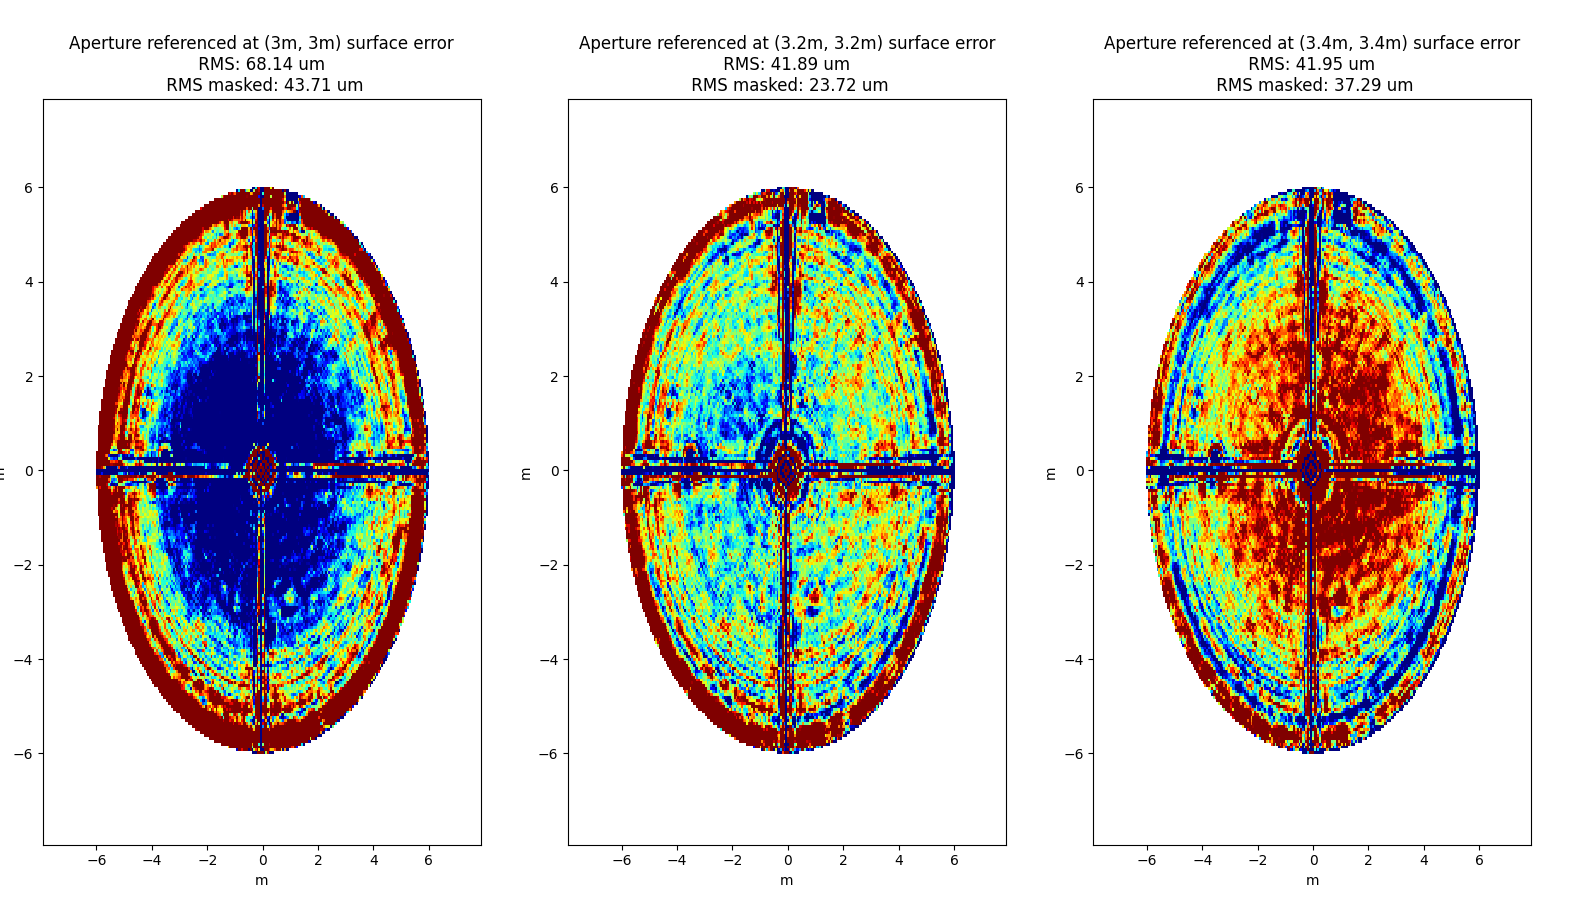
\includegraphics[width=1\textwidth]{images/phase_zero_example.png}
    \caption{Effect on the surface error maps of the phase zero setting on aperture plane.}
    \label{fig:phase_zero_ex}
\end{figure}








\section{Large Scale removal}


\subsection{Zernike polynomials fitting at the aperture}
The Zernike fitting its done in the aperture with the magnitude and phase values. The representation follows the one used in \cite{cassanelli_oof} where the aperture is model as the equation \ref{eq:oof_aperture} where the $B$ term represents the blockage of the telescope, $E(x,y)$ is the illumination and $\phi_z$ represents the large scale errors using the Zernike polynomials as the equation \ref{eq:oof_zernike_errors}, where the $k_{m,n}$ term are the coefficient of each Zernike polynomial.




\begin{equation}
    f(x,y) = B(x,y)E(x,y)e^{i k \phi_z(x,y)}
    \label{eq:oof_aperture}
\end{equation}

\begin{equation}
    \phi_z(x,y) =  \sum_n \sum_m k_{n,m}U^{m}_{n}(\rho, \theta)
    \label{eq:oof_zernike_errors}
\end{equation}


Then for a given radial order $n$ there will be $(n+1)(n+2)/2$ coefficients that needs to be fitted. 
For simplicity we take an uniform illumination and the mask is given by the telescope geometry, with this setup we are only adding 1 more parameter to the optimization process that is the amplitude of the illumination. In principle the illumination function can be changed for any other function, as gaussian or parabolic illumination, but this would add more parameters to the fitting procedure.


The main advantage of using the Zernike fitting is that the contribution of each optical aberration can be separated from the rest and you can determine if the telescope has an optical issue. The drawbacks are that the compuation time is longer than other methods since the optimization process is done in complex values.

\subsection{Polynomial fitting at the surface error}

The second method implemented consists of using a 2D polynomial function composed by the $(x,y)$ coefficients. So for a given order $N$ the function takes the form shown in equation \ref{eq:pol_surf}, where the number of coefficients to be found is $(N+1)(N+2)/2$. 


\begin{gather}
    p(x,y) = \sum_{m=0}^{n-1}\sum_{n=0}^{N-1} c_{n, m} x^{n}y^{m} =\\ 
    c_{00}+c_{10}x+\dots+c_{N0}x^{N-1}+c_{01}y+\cdots+c_{0N}y^{N-1}+c_{11}xy+c_{12}x^1y^2+\cdots
    \label{eq:pol_surf}
\end{gather}

This polynomial fitting is done in the surface of the antenna, so its a real value fitting and its way faster than the Zernike optimization. This surface fitting also considers the blockage of the suporting legs and the subreflector.
The drawback of this method is that you cannot separate the effects of different types of aberrations.


\subsection{Comparison of the methods}

Since both models have similar number of parameters for a given degree (when having uniform illumination the Zernike model has 1 extra parameter compared with the polynomial fitting, the one comming from the illumination) we can compare the fitting results of the two methods. To make a fair comparison the Zernike polynomial result is translated to the antenna surface error. The example map used to compare the methods is the output of the nearfield corrected stage, shown in \ref{fig:nearfield_correction}.
The figures \ref{fig:large_scale_comp_2}, \ref{fig:large_scale_comp_3}, \ref{fig:large_scale_comp_4} and \ref{fig:large_scale_comp_5} shows the comparison of the models generated when removing the large scale errors for different depolynomial degrees. As can be seen the resuults are quite similar and shows the same structures for a given degree. 
For this example the Zernike coefficients with degree 4 are shown in the table \ref{table:zernike_modes}.


\begin{table}[]
    \label{table:zernike_modes}
    \centering
    \caption{Resulting zernike coefficients for the degree=4.}
\begin{tabular}{|l|l|l|}
\hline
Zernike mode & name                         &  value  \\ \hline
n=0,         & Piston                       &  1.25e-5 \\ \hline
n=1,m=-1     & Vertical tilt                &  -5.7e-7 \\ \hline
n=1,m=1      & Horizontal tilt              &  1.2e-5   \\ \hline
n=2,m=-2     & Oblique astigmatism          &  -1.e-5   \\ \hline
n=2,m=0      & Defocus                      &  -2.6e-5   \\ \hline
n=2,m=2      & Vertical astigmatism         &  -7.e-6   \\ \hline
n=3,m=-3     & Vertical trefoil             &  -4.2e-6   \\ \hline
n=3,m=-1     & Vertical coma                &  -1.6e-6   \\ \hline
n=3,m=1      & Horizontal coma              &  4.1e-5   \\ \hline
n=3,m=3      & Oblique trefoil              &  5.1e-6   \\ \hline
n=4,m=-4     & Oblique quadrafoil           &  5.5e-6   \\ \hline
n=4,m=-2     & Oblique second astigmatism   &  -3.7e-6   \\ \hline
n=4,m=0      & Primary spherical            &  3.6e-5   \\ \hline
n=4,m=2      & Vertical second astigmatism  &  -2.4e-6   \\ \hline
n=4,m=4      & Vertical quadrafoil          &  -1.3e-5   \\ \hline
\end{tabular}
\end{table}




\begin{figure}
    \centering
    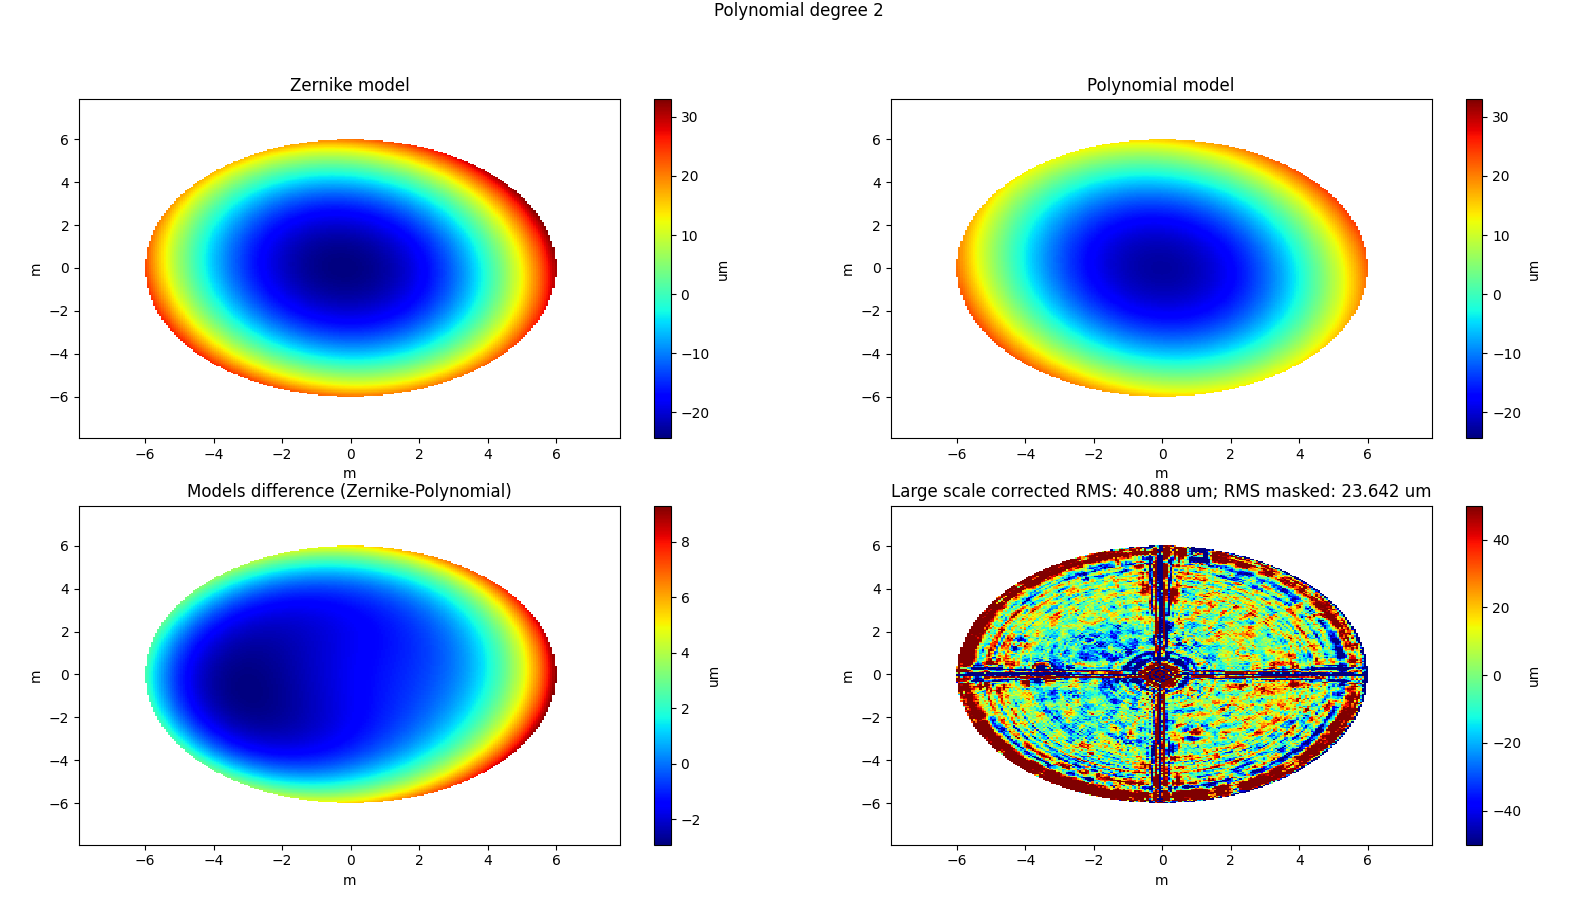
\includegraphics[width=0.9\textwidth]{images/large_scale_comp_2.png}
    \caption{Comparison of both large scale removal methods when using a degree 2 polynomial (6 parameters)}
    \label{fig:large_scale_comp_2}
\end{figure}


\begin{figure}
    \centering
    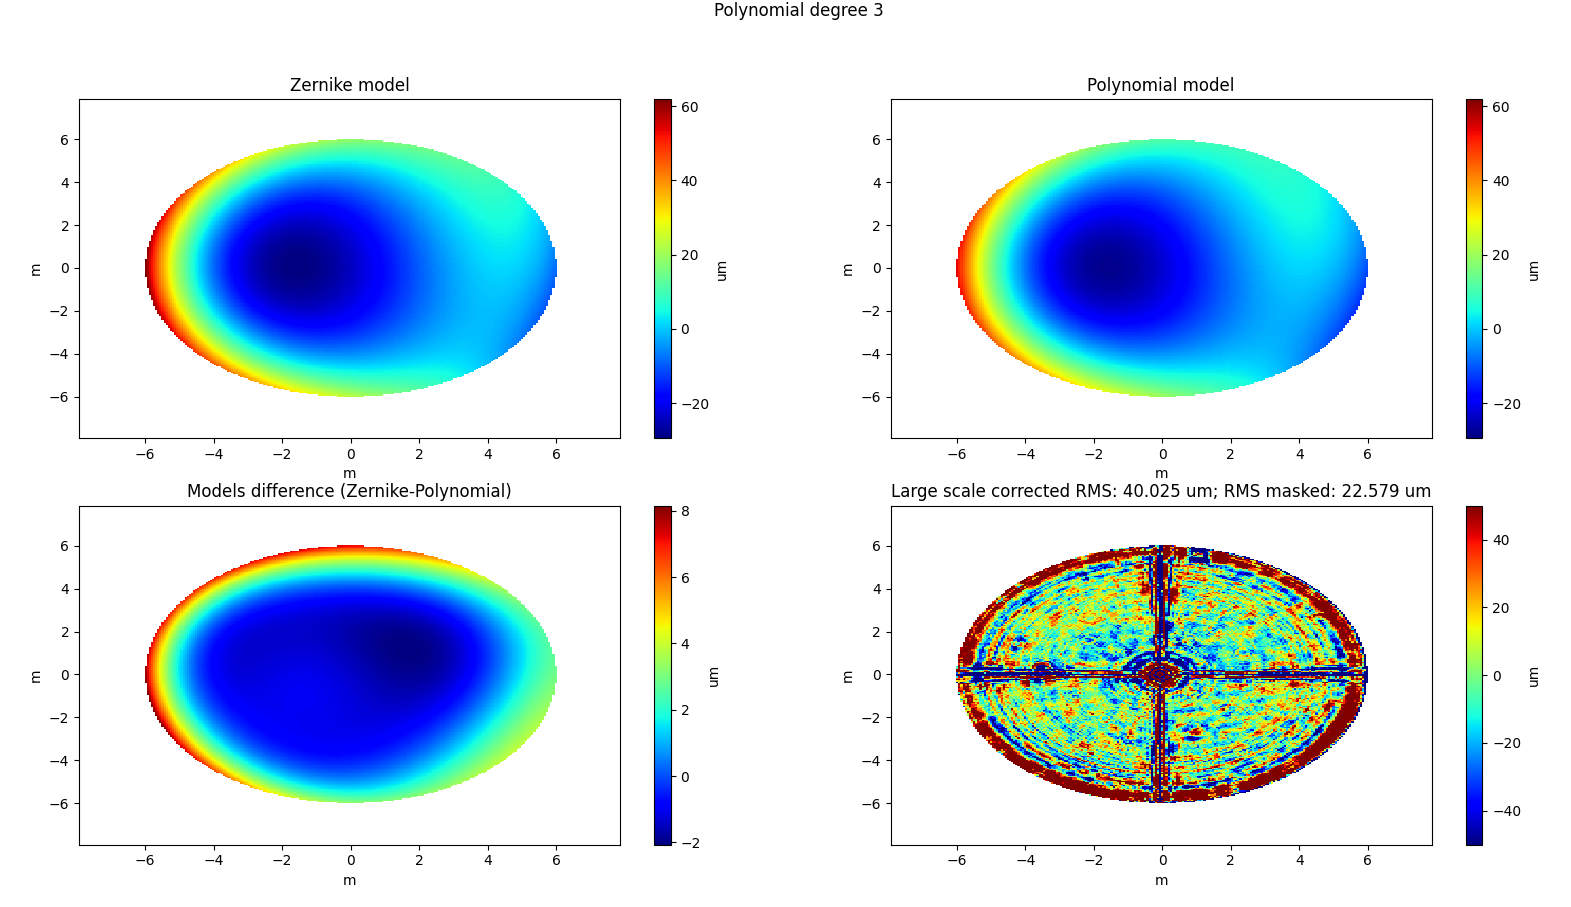
\includegraphics[width=0.9\textwidth]{images/large_scale_comp_3.png}
    \caption{Comparison of both large scale removal methods when using a degree 3 polynomial (10 parameters)}
    \label{fig:large_scale_comp_3}
\end{figure}



\begin{figure}
    \centering
    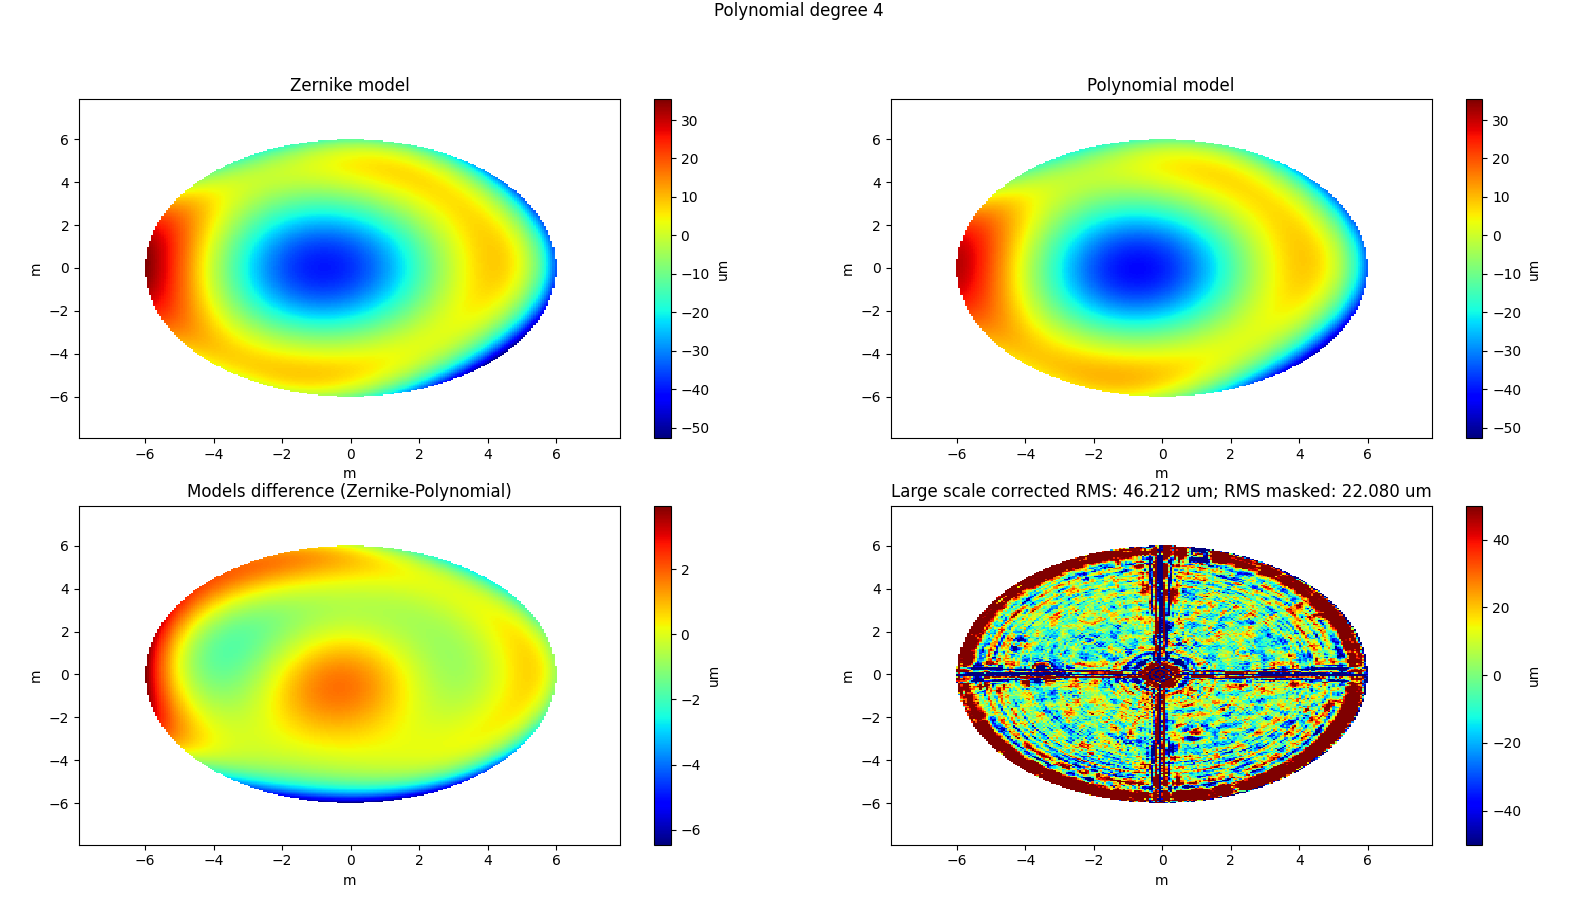
\includegraphics[width=0.9\textwidth]{images/large_scale_comp_4.png}
    \caption{Comparison of both large scale removal methods when using a degree 4 polynomial (15 parameters)}
    \label{fig:large_scale_comp_4}
\end{figure}


\begin{figure}
    \centering
    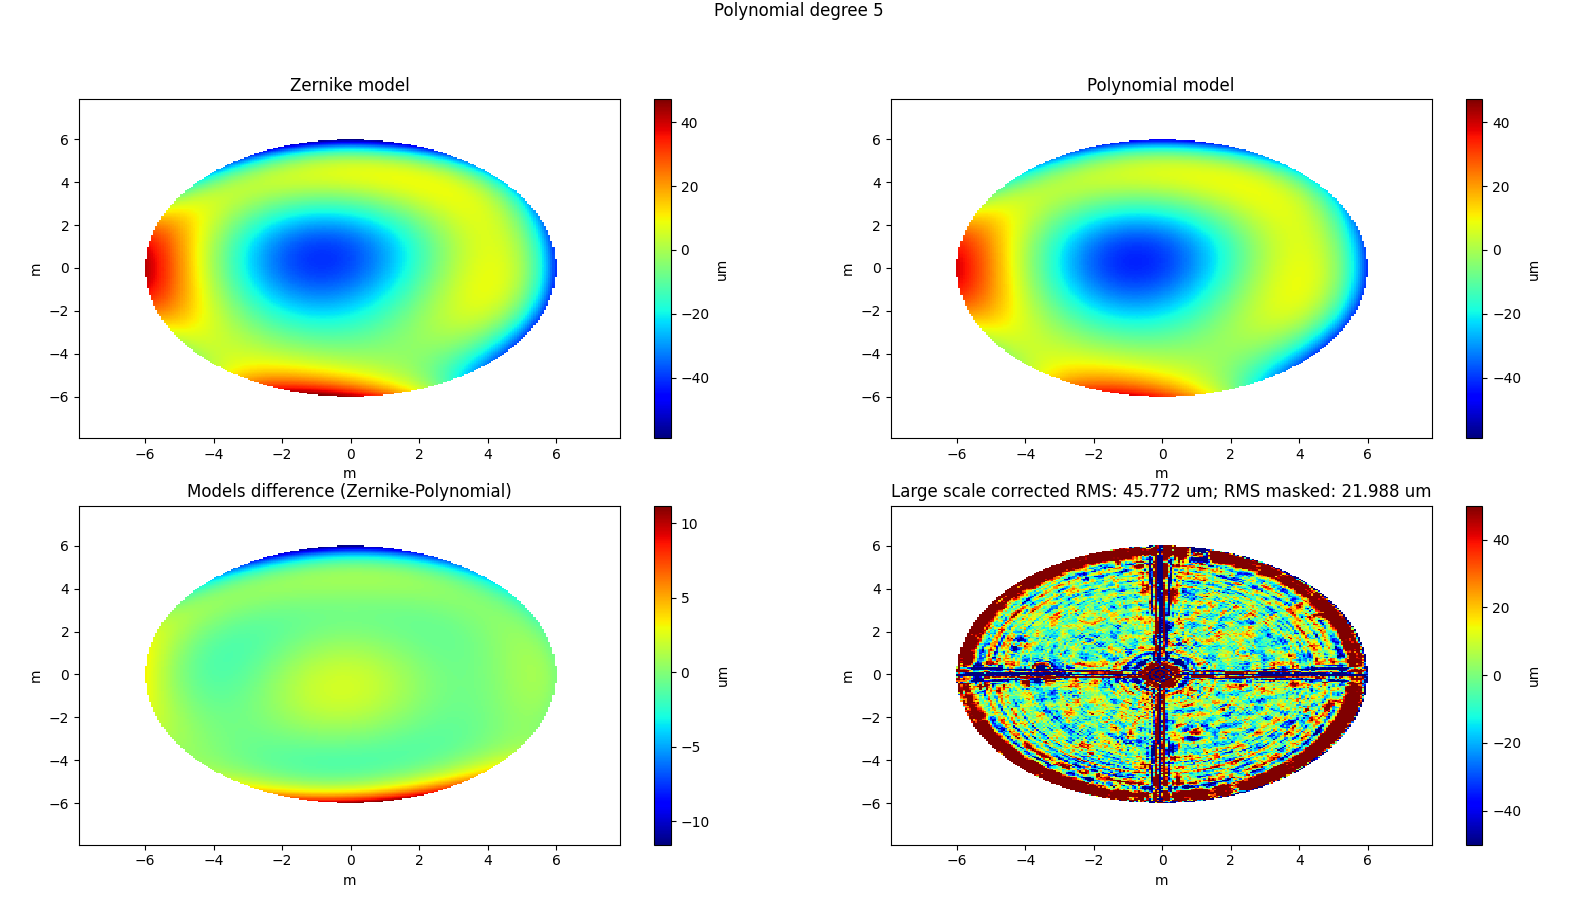
\includegraphics[width=0.9\textwidth]{images/large_scale_comp_5.png}
    \caption{Comparison of both large scale removal methods when using a degree 5 polynomial (21 parameters)}
    \label{fig:large_scale_comp_5}
\end{figure}










\newpage
\section{Diffraction substraction}

To account the diffraction produced by the secondary a model in the GRASP software was made using the APEX telescope parameters.
The result was transformed to the surface error and scaled to match a grid of 256x256 pixels that is the common pixel size used in APEX holography pipelines. If a map of different pixel size is used a 2D interpolation is made to match the map size.

The figure \ref{fig:grasp_diffraction} shows the GRASP diffraction model, this model is substracted from the large scale corrected map. The figure \ref{fig:diffraction_corrected} shows the effect of the diffraction model substraction.


\begin{figure}
    \centering
    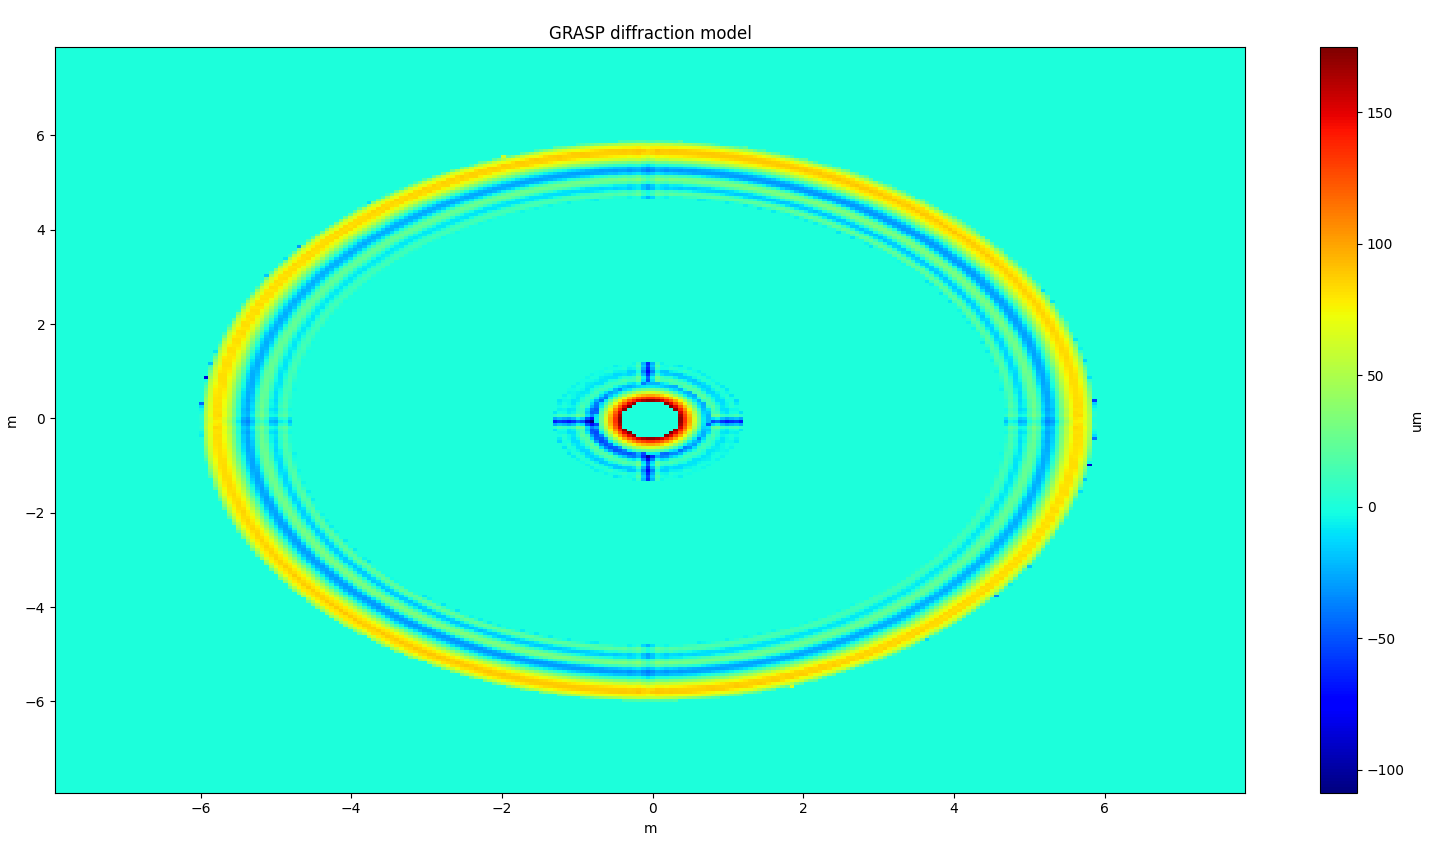
\includegraphics[width=0.8\textwidth]{images/grasp_diffraction_model.png}
    \caption{GRASP diffraction model.}
    \label{fig:grasp_diffraction}
\end{figure}


\begin{figure}
    \centering
    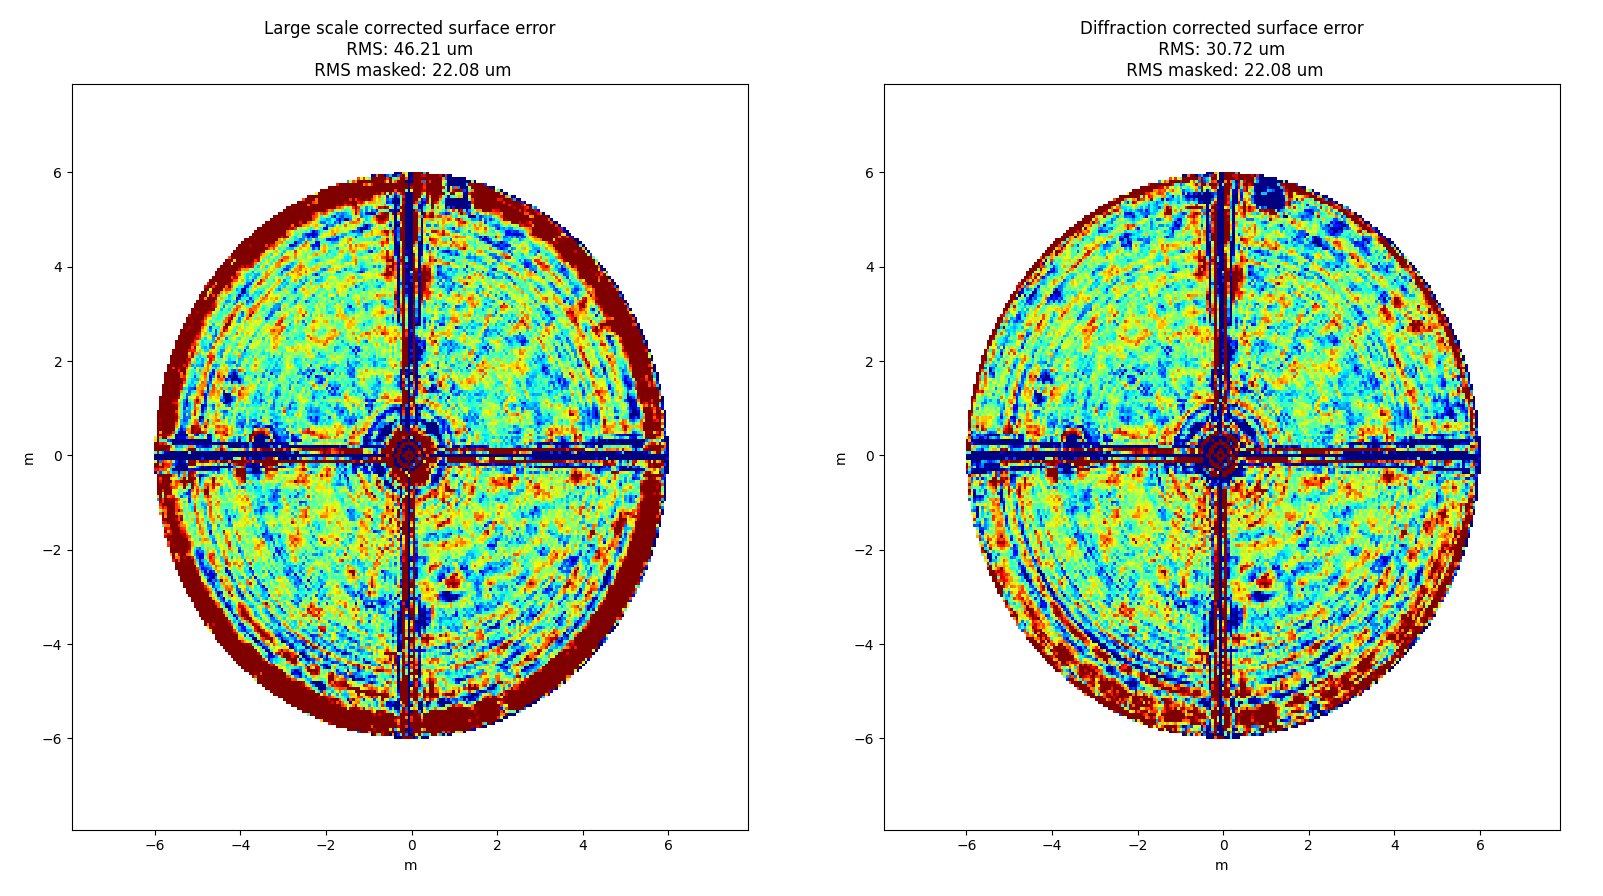
\includegraphics[width=0.9\textwidth]{images/diffraction_correction.png}
    \caption{Example of the effect of the substraction of the diffraction model.}
    \label{fig:diffraction_corrected}
\end{figure}



\subsection{Supporting legs substraction}

To account the effect on the supporting legs a more practical approach was taken. We devided the total radius of the dish in different zones, eg: $[0.375, 1.75, 3.,4.5, 6]$. Since we are going to assume axial symmetry along the vertical and horizontal axis, we separate the effect of the legs placed vertically and the ones placed horizontally.

As an example we are going to take the X axis and the radius region $[0.375, 1.75[$ and considering the legs width as $0.4m$, we have two regions to consider: the one at $A1=(-1.75,0.2), (-0.375,0.2), (-0.375, -0.2), (-1.75,-0.2)$ and $A2=(0.375,0.2), (1.75, 0.2), (1.75, -0.2), (0.375,-0.2)$ as show in the figure \ref{fig:ex_legs_region}. As this example is in the X axis, we will move in the Y direction and for each Y value we will compute the median (or average) of the pixels at that heigh (from both regions $A1$ and $A2$) and this value will be the correction for all the pixels at that height.


For the case of Y axis, the median (or average) computation will be at each X value.
The figure \ref{fig:legs_removal} shows the final model result and the effect iof its substraction, the input map used to obtain these figures is the same one obtained from the diffraction model correction shown in \ref{fig:diffraction_corrected}.

\begin{figure}
    \centering
    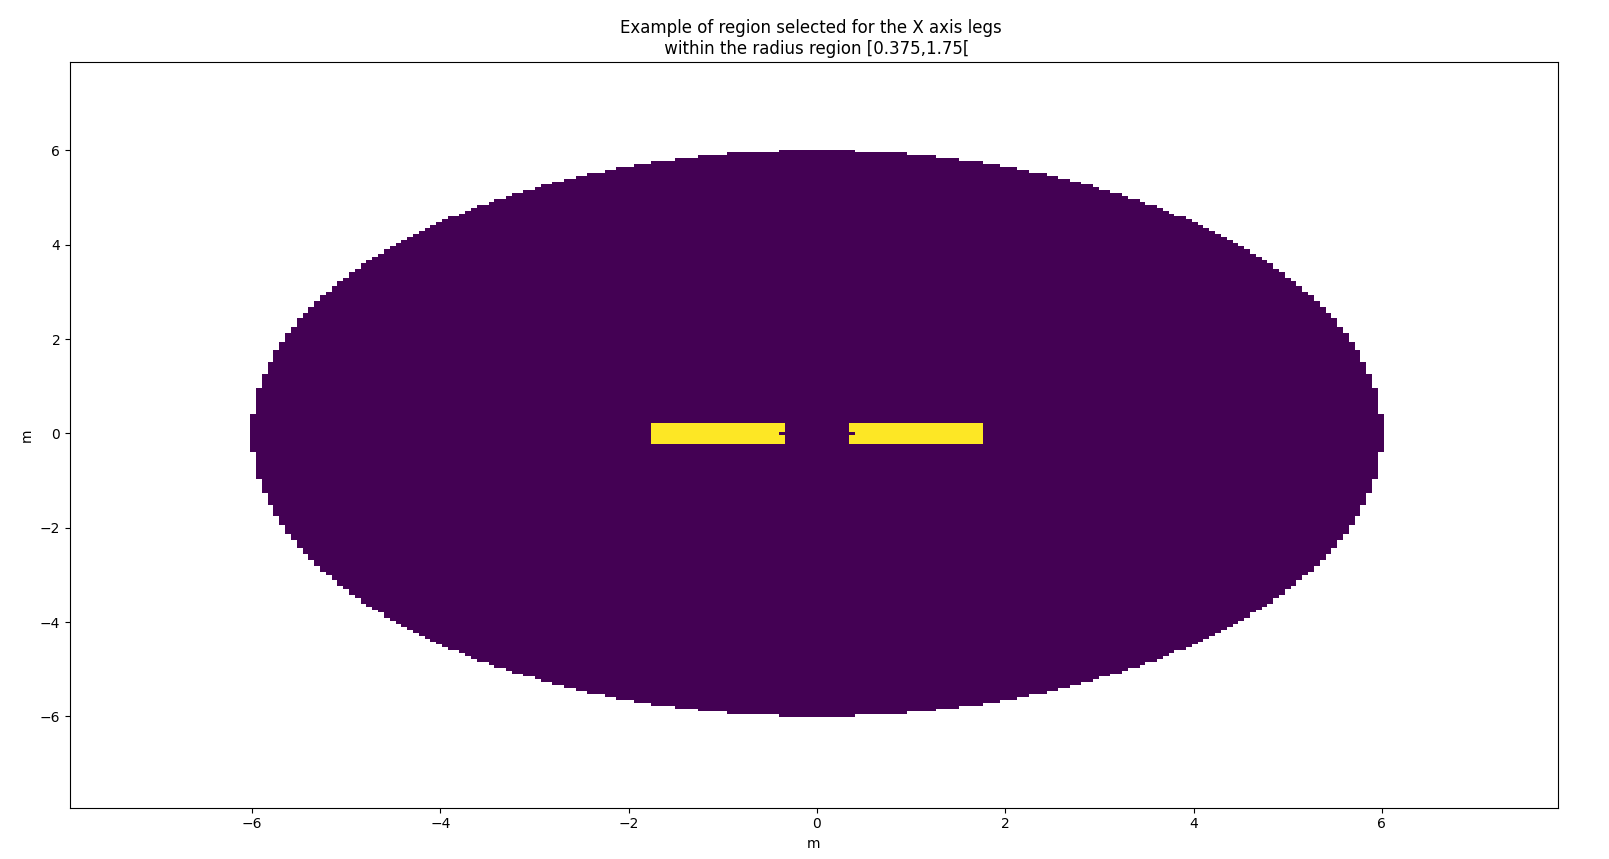
\includegraphics[width=0.9\textwidth]{images/ex_legs_region.png}
    \caption{Example of the regions selected for X axis supporting legs within the radius $[0.375,1.75[$.}
    \label{fig:ex_legs_region}
\end{figure}


\begin{figure}
    \centering
    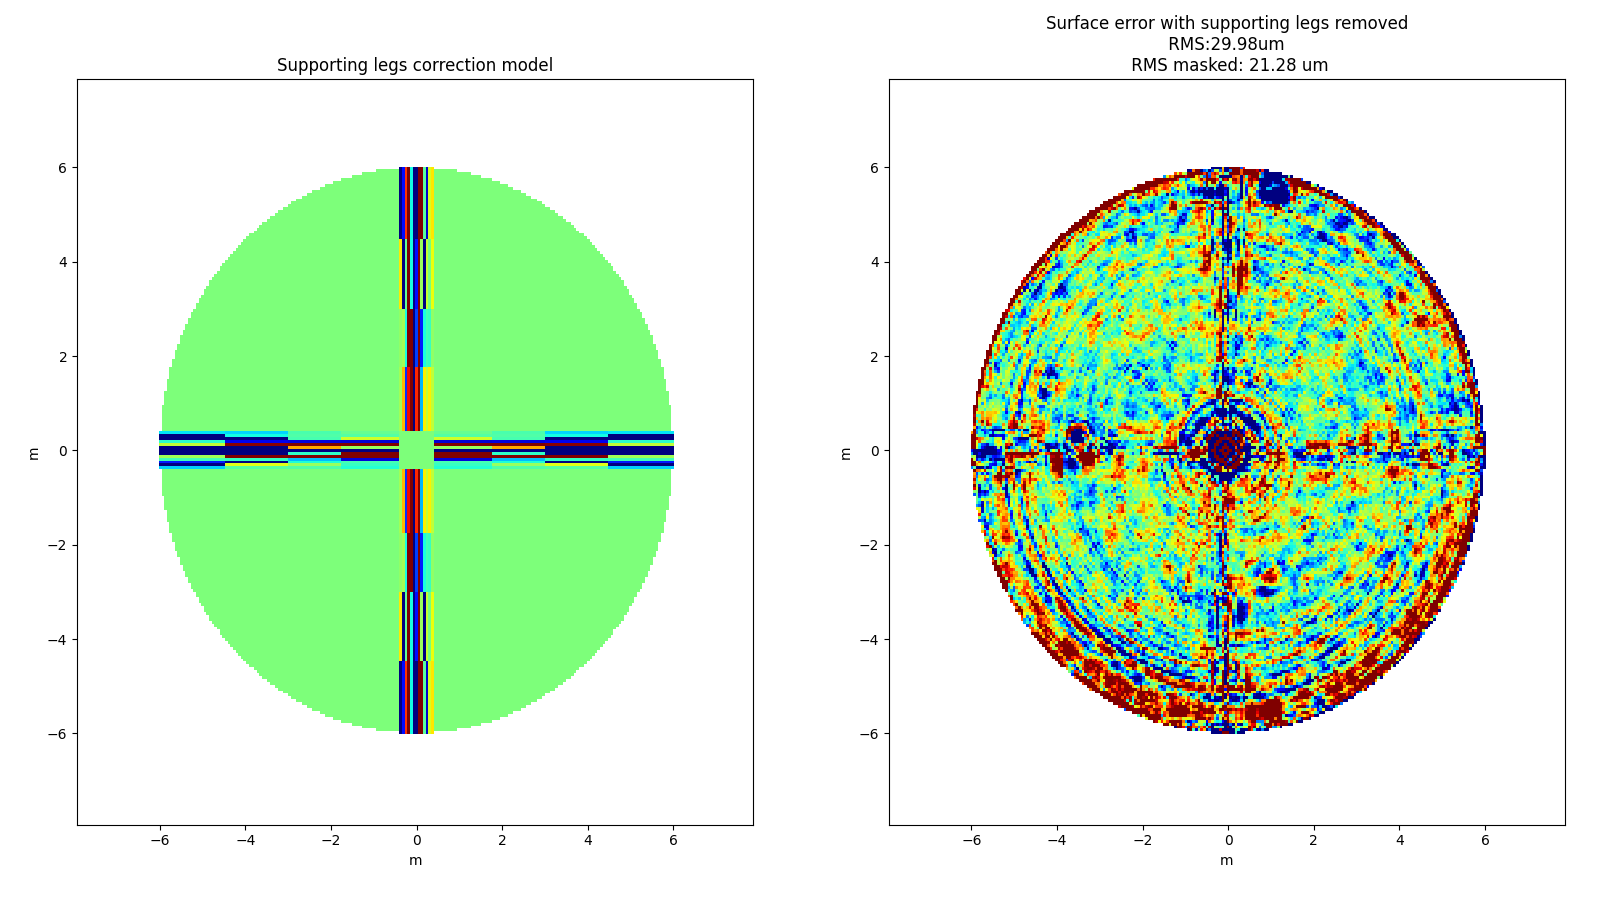
\includegraphics[width=0.9\textwidth]{images/legs_removal.png}
    \caption{Supporting legs model and the resulf of its removal in the surface error map.}
    \label{fig:legs_removal}
\end{figure}







\section{Panel fitting}




\section{Results statistics}

To detect the repetibility of the adjustments predicted by the reduction pipeline we select a set of maps taken in the same date to have similar conditions.
For each map we run the complete pipeline and we compare the screws adjustments between the maps. As we dont know the true optimal adjustment, we would only care about the variability of the results.
The maps selected are shown in the figure \ref{fig:statistic_maps} and the figure \ref{fig:hist_example} shows the difference in the screws adjustment heights predicted for different maps that were taken in the same night.

\begin{figure}
    \centering
    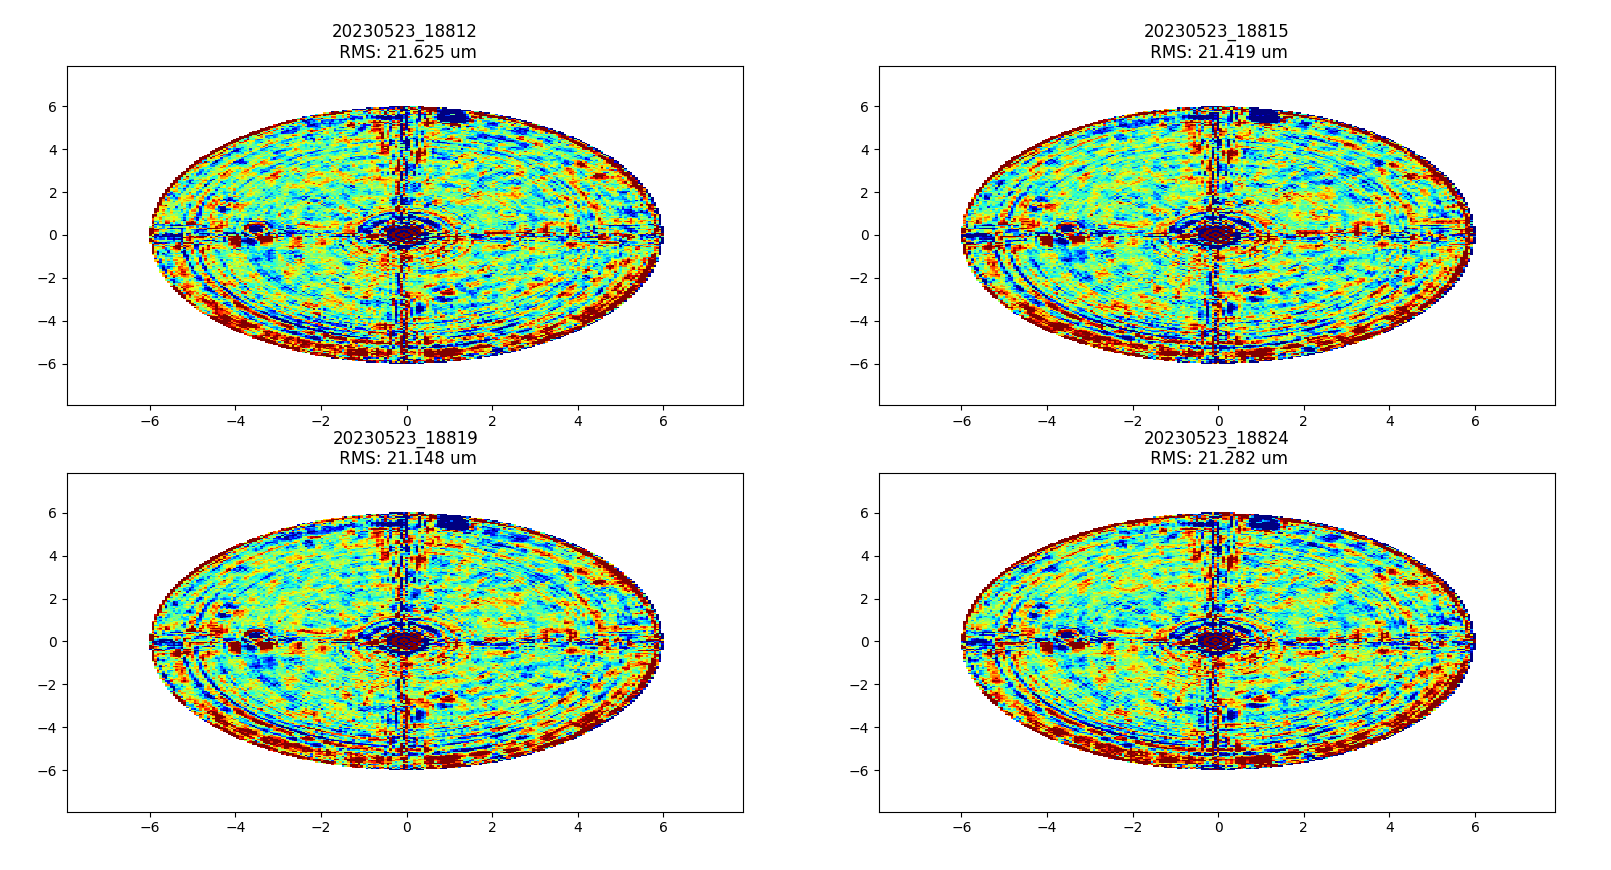
\includegraphics[width=\textwidth]{images/20230523_maps.png}
    \caption{Selected maps for the variability study. These maps are part of a single night measurement, so the conditions when making the maps were comparable.}
    \label{fig:statistic_maps}
\end{figure}



\begin{figure}
    \centering
    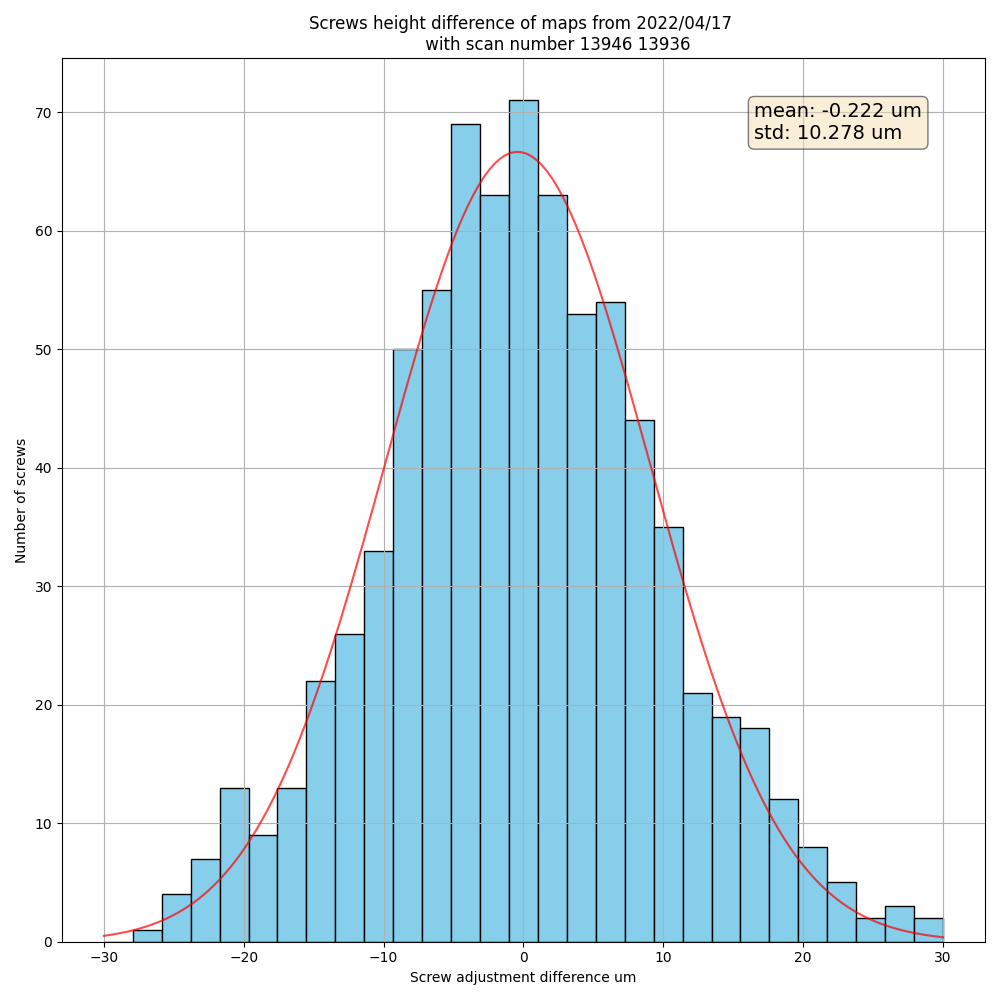
\includegraphics[width=0.6\textwidth]{images/hist_example.png}
    \caption{Example of the obtained histogram when comparing the screws heights values that the pipeline compute for each map.}
    \label{fig:hist_example}
\end{figure}



The histogram plot shows that the difference between the set of screw adjustments can be well represented by a normal distribution where, in a non-rigourous way, the average value can be thoughit as a global piston difference between the two sets and the standard deviation is the measurement variability and its the parameters that we are interested in.

As we do not know the true value of the adjustment we can only make pairwise comparison, considering on of the predictions as true. This can be summarized in the confusion matrix shown in figures \ref{fig:conf_matrix_plane} where for every row the screws adjustment of that map are consider as the true values and compared with the rest maps. Each one of these comparison lead to a distribution like the one shown in figure \ref{hist_example}, the confusion matrix summarize gaussian parameters of every distribution.


The confusion matrix in the figure \ref{fig:conf_matrix_plane} shows the results when using the pure plane panel fitting method, whereas the figure \ref{fig:cong_matrix_deform} use the deformed plane panel fitting.

From these results we can tell that we got a variability around $7-8\mu m$ in the adjustments, so the error that we have in the adjusted surface has that as a lower bound (this is a systematic error, so there are more sources of errorrs, and the final surface error should be higher).


\begin{figure}
    \centering
    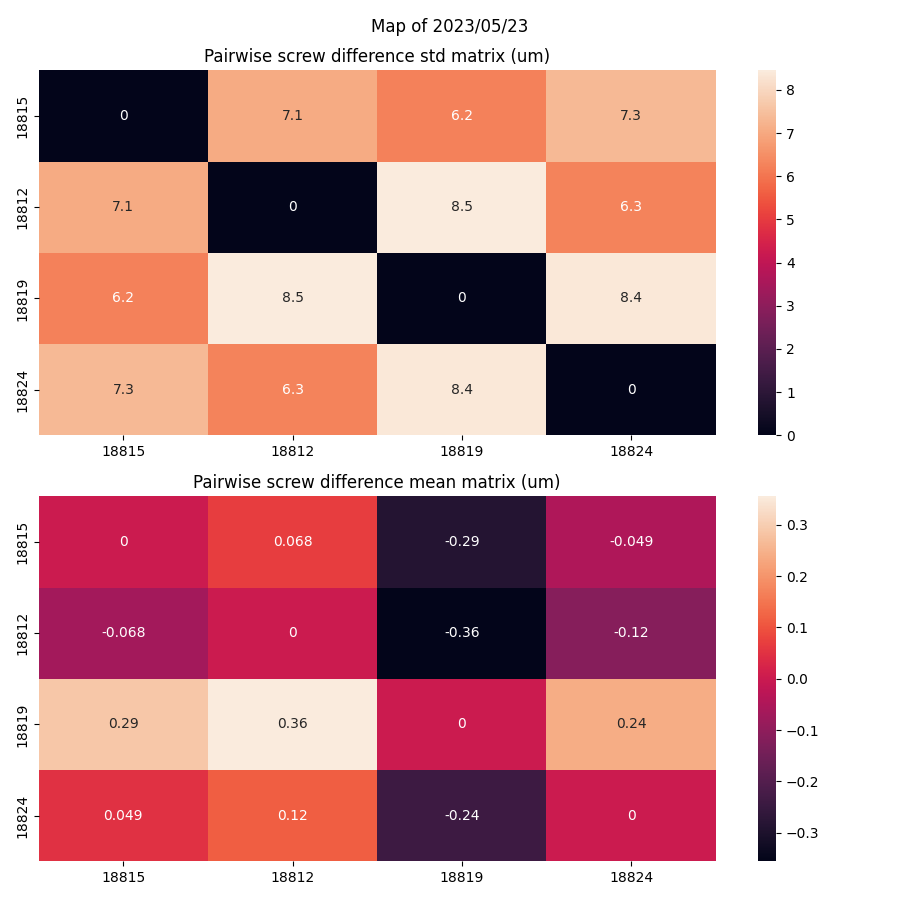
\includegraphics[width=0.8\textwidth]{images/20230523_mat_panelfit_plane.png}
    \caption{Confusion matrix of the maps with the pure plane panel fitting method to compute the screws adjustments.}
    \label{fig:conf_matrix_plane}
\end{figure}

\begin{figure}
    \centering
    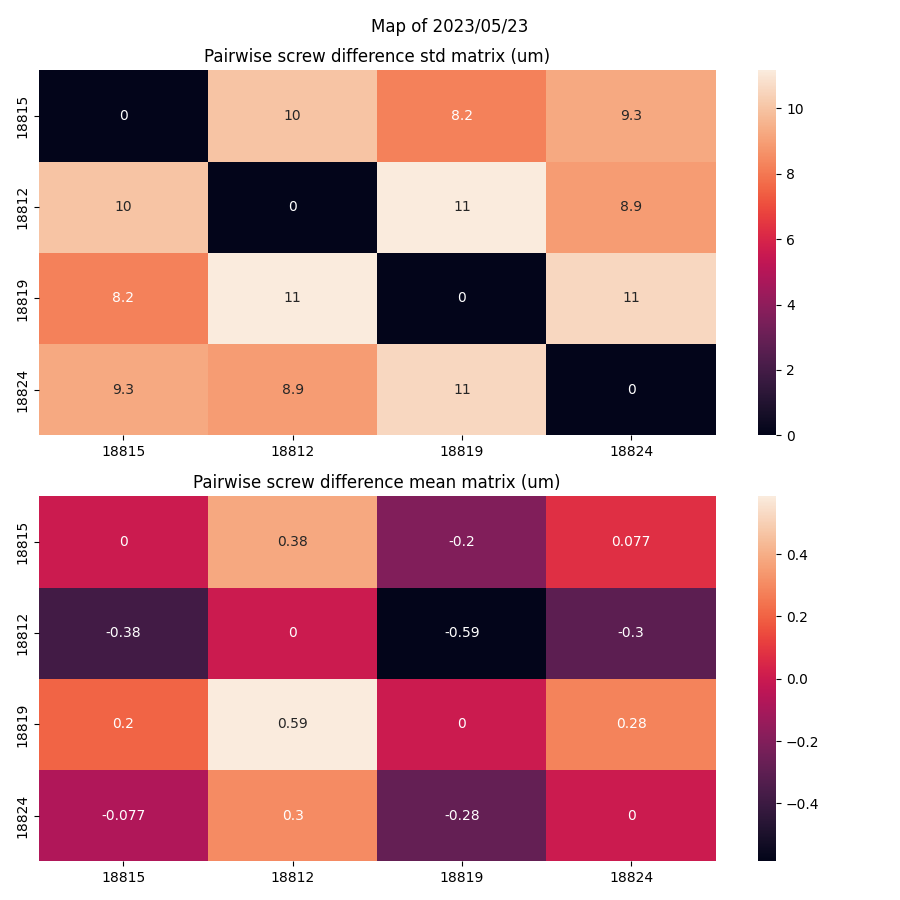
\includegraphics[width=0.8\textwidth]{images/20230523_mat_panelfit_deform.png}
    \caption{Confusion matrix of the maps with the deformed plane panel fitting method to compute the screws adjustments.}
    \label{fig:conf_matrix_deform}
\end{figure}






\bibliographystyle{ieeetr}
\bibliography{references}

\end{document}
